%%%%%%%%%%%%%% 05/03/2020 %%%%%%%%%%%%%%%% 
\subsection*{05/03/2020}
\subsubsection{Day aims}
\begin{itemize}
    \item Finish calculation of uncertainty for $Z \rightarrow ee$ and $Z \rightarrow \mu\mu$
\end{itemize}

\subsubsection{Day Summary}
\begin{itemize}
    \item Considered transverse momentum and isolation variables for individual leptons
    \item Made finalisations on Z process cuts
    
\end{itemize}
%%%%%%%%%%%%%% 09:54 %%%%%%%%%%%%%%%% 
\subsubsection*{09:54 - PT of single leptons (Higgss)}
Plotting the transverse lepton transverse momentum for lepton 0 ($lep_pt[0]$) and for lepton 3 on different plots ((A) and (B) respectively).
\\
lepton [0] should have lower transverse momentum than lepton [3]
\\
Cuts used in Fig.\ref{}:
\begin{lstlisting}
    ...
\end{lstlisting}
\begin{figure}[h!]
    \centering
    \begin{minipage}{0.5\textwidth}
        \centering
        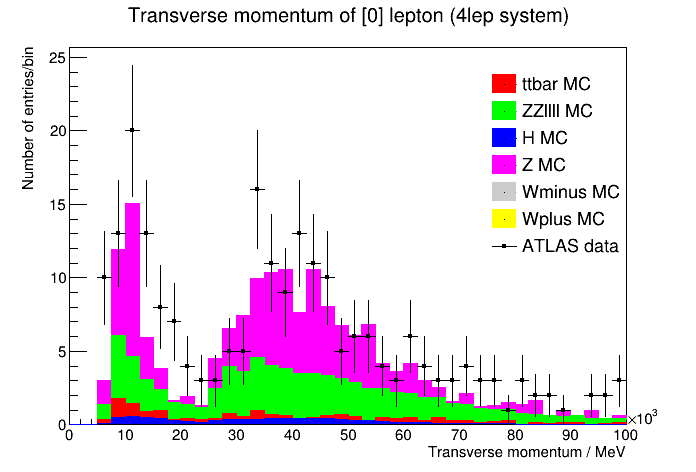
\includegraphics[width=\linewidth]{plots/05-03-2021/09-54_05-03.png}
        (A)
    \end{minipage}\hfill
    \begin{minipage}{0.5\textwidth}
        \centering
        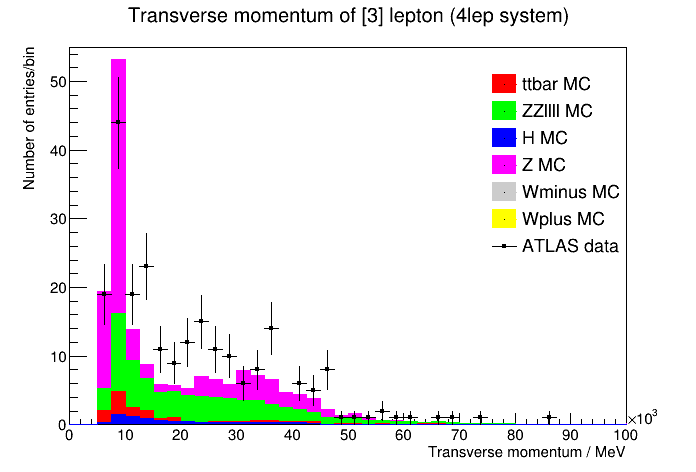
\includegraphics[width=\linewidth]{plots/05-03-2021/10-32_05-03-21.png}
        (B)
    \end{minipage}
    \caption{(A) Transverse momentum of lepton [0] of the 4 lepton system. (B) Transverse momentum of lepton [3] of the 4 lepton system. Includes ATLAS data with H MC signal simulation data, and background MC data.  Cuts: lep-n == 4, only allowed end products: == e+e- mu+mu-, e+e-e+e-, mu+mu- mu+mu-, with one lepton pair with invariant mass of $60 GeV < m_{ll} < 150 GeV$ and the other $m_{ll} < 60 GeV$}
    \label{fig}
\end{figure}


%%%%%%%%%%%%% 10:20 %%%%%%%%%%%%%
\subsubsection*{10:20 - Plotting the PT for $\mu\mu$ (with full cuts)}
Plotting the transverse momentum for $Z \rightarrow \mu\mu$ as a stack plot (fast).
\\
Cuts used in Fig.\ref{fig:10-20_03-03-21}:
\begin{lstlisting}
basic_cut = "(lep_charge[0] != lep_charge[1]) && (lep_type[0] == 13 && lep_type[1] == 13) && lep_n==2"

inv_mass_cut = "(inv_mass_Zll > 70e3) && (inv_mass_Zll < 150e3)"

etcone_cut = "(lep_etcone20[0] > -2e3 && lep_etcone20[1] > -2e3)" + "&& (lep_etcone20[0] < 6e3 && lep_etcone20[1] < 6e3)"

ptcone_cut = "(lep_ptcone30[0] < 5.8e3) && (lep_ptcone30[1] < 5.8e3)"

lepCut = "(" + basic_cut + "&&" + inv_mass_cut + "&&" + etcone_cut + "&&" + ptcone_cut + ")"

t.SetAlias("inv_mass_Zll","sqrt(2*lep_pt[0]*lep_pt[1]*(cosh(lep_eta[0]-lep_eta[1])-cos(lep_phi[0]-lep_phi[1])))")

t.Draw("lep_pt[1] >> h_lep_pt_total(100, 0,100e3)", weighting + "*" + lepCut)
\end{lstlisting}

\begin{figure}[h!]
    \centering
    \begin{minipage}{0.5\textwidth}
        \centering
        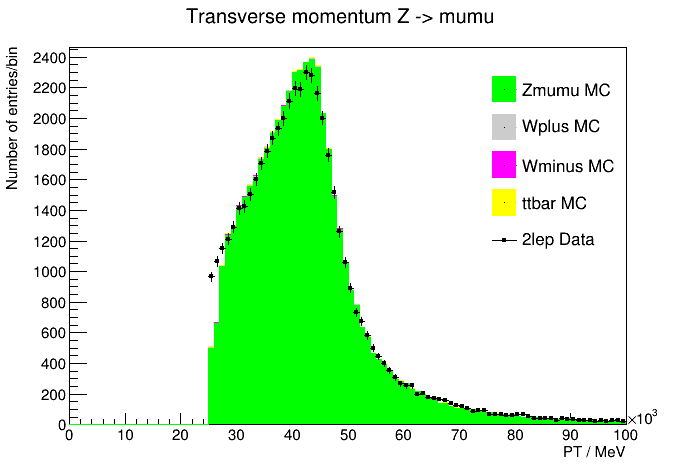
\includegraphics[width=\linewidth]{plots/03-03-2021/10-20_03-03-21.png}
        (A)
    \end{minipage}\hfill
    \begin{minipage}{0.5\textwidth}
        \centering
        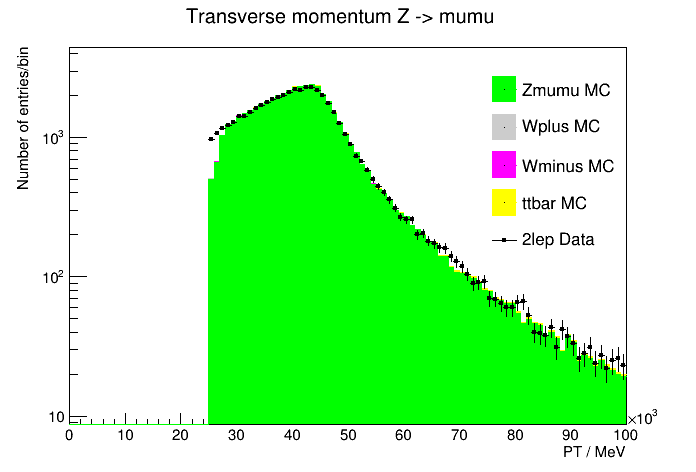
\includegraphics[width=\linewidth]{plots/03-03-2021/10-21_03-03-21.png}
        (B) 
    \end{minipage}
    \caption{(A) Transverse momentum of mumu pair with ATLAS, Signal, and background MC data. (B) Transverse momentum of mumu pair with ATLAS, Signal, and background MC data - log-y plot.  Cuts: electron pair with opposite charge, $70 GeV < m_{\mu\mu} < 150 GeV$, $36 GeV < p_T$, $ ptcone < 5.8 GeV$, $ -2 GeV < etcone < 6 GeV$.}
    \label{fig:10-20_03-03-21}
\end{figure}

Cuts for $Z \rightarrow \mu\mu$:
\begin{align}
    p_T > 28 GeV    
\end{align}

%%%%%%%%%%%%% 11:00 %%%%%%%%%%%%%
\subsubsection*{11:00 - Plotting $m_{ll}$ for mumu (with full cuts)}
Plotting the invariant mass for $Z \rightarrow \mu\mu$ as a stack plot (fast).
\\
Cuts used in Fig.\ref{fig:11-00_03-03-21}:
\begin{lstlisting}
basic_cut = "(lep_charge[0] != lep_charge[1]) && (lep_type[0] == 13 && lep_type[1] == 13) && lep_n==2"
   
etcone_cut = "(lep_etcone20[0] > -1.6e3 && lep_etcone20[1] > -1.6e3)" + "&& (lep_etcone20[0] < 5.25e3 && lep_etcone20[1] < 5.25e3)"

ptcone_cut = "(lep_ptcone30[0] < 6.5e3) && (lep_ptcone30[1] < 6.5e3)"

pt_cut = "(lep_pt[0] > 28e3) && (lep_pt[1] > 28e3)"
    
lepCut = "(" + basic_cut + "&&" + inv_mass_cut + "&&" + etcone_cut + "&&" + ptcone_cut + "&&" + pt_cut + ")"

t.SetAlias("inv_mass_Zll","sqrt(2*lep_pt[0]*lep_pt[1]*(cosh(lep_eta[0]-lep_eta[1])-cos(lep_phi[0]-lep_phi[1])))")
  
t.Draw("inv_mass_Zll >> h_inv_mass(100,0,150e3)", weighting + "*" + lepCut)
\end{lstlisting}
\begin{figure}[h!]
    \centering
    \begin{minipage}{0.5\textwidth}
        \centering
        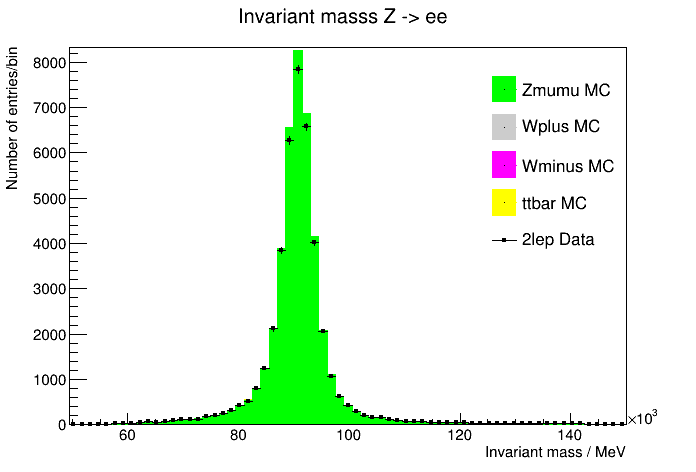
\includegraphics[width=\linewidth]{plots/03-03-2021/11-01_03-03-21.png}
        (A)
    \end{minipage}\hfill
    \begin{minipage}{0.5\textwidth}
        \centering
        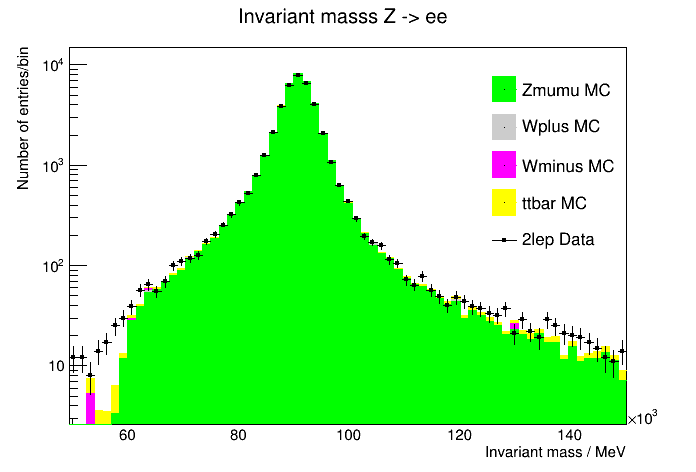
\includegraphics[width=\linewidth]{plots/03-03-2021/11-00_03-03-21.png}
        (B)
    \end{minipage}
    \caption{(A) Invariant mass of mumu pair with ATLAS, Signal, and background MC data. (B) Transverse momentum of mumu pair with ATLAS, Signal, and background MC data - log-y plot.}
    \label{fig:11-00_03-03-21}
\end{figure}

Cuts made on invariant mass for mumu:
\begin{align}
    65 GeV < m_{\mu\mu} < 150 GeV
\end{align}


%%%%%%%%%%%%% 11:20 %%%%%%%%%%%%%
\subsubsection*{11:20 - Estimation of systematic uncertainty using variations in PTcone for $\sigma (Z \rightarrow \mu\mu)$}
Plot of PTCone with the full cuts: (Fig.\ref{fig:11:00_05-03-21})
\begin{lstlisting}
basic_cut = "(lep_charge[0] != lep_charge[1]) && (lep_type[0] == 13 && lep_type[1] == 13) && lep_n==2"
 
inv_mass_cut = "(inv_mass_Zll > 65e3) && (inv_mass_Zll < 150e3)"

etcone_cut = "(lep_etcone20[0] > -1.6e3 && lep_etcone20[1] > -1.6e3)" + "&& (lep_etcone20[0] < 5.25e3 && lep_etcone20[1] <5.25e3)"

pt_cut = "(lep_pt[0] > 28e3) && (lep_pt[1] > 28e3)"
    
lepCut = "(" + basic_cut + "&&" + pt_cut + "&&" + inv_mass_cut + "&&" + etcone_cut + ")"

t.SetAlias("inv_mass_Zll","sqrt(2*lep_pt[0]*lep_pt[1]*(cosh(lep_eta[0]-lep_eta[1])-cos(lep_phi[0]-lep_phi[1])))")
   
t.Draw("lep_ptcone30[0] >> h_lep_ptcone30(100,0e3,7e3)", weighting + "*" + lepCut)
\end{lstlisting}
\begin{figure}[h!]
    \centering
	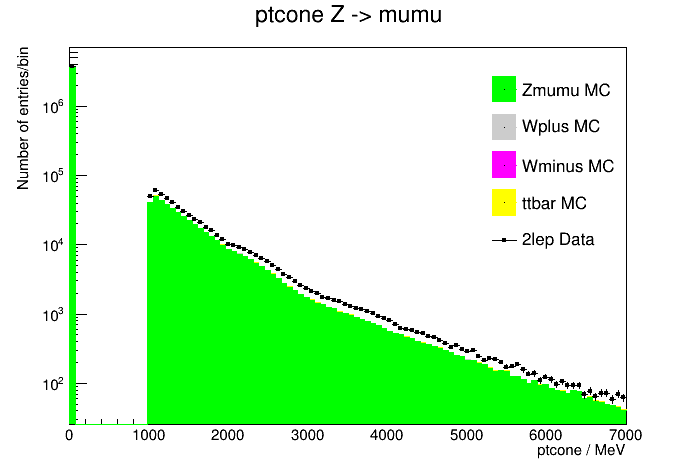
\includegraphics[width=0.85\linewidth]{plots/05-03-2021/11-20_05-03-21.png}
    \caption{PTCone with full cuts:}
    \label{fig:11:00_05-03-21}
\end{figure}
Fig.ref{} shows the cross section for various upper bounds on the ptcone
\\
Estimation of cross section and uncertainty:

%%%%%%%%%%%%% 12:08 %%%%%%%%%%%%%
\subsubsection*{12:08 - Estimation of systematic uncertainty using variations in ETcone for $\sigma (Z \rightarrow \mu\mu)$}
% 11-30_05-03-21.png
\begin{lstlisting}
basic_cut = "(lep_charge[0] != lep_charge[1]) && (lep_type[0] == 13 && lep_type[1] == 13) && lep_n==2"

inv_mass_cut = "(inv_mass_Zll > 65e3) && (inv_mass_Zll < 150e3)"

ptcone_cut = "(lep_ptcone30[0] < 6.5e3) && (lep_ptcone30[1] < 6.5e3)"

pt_cut = "(lep_pt[0] > 28e3) && (lep_pt[1] > 28e3)"
 
    
lepCut = "(" + basic_cut + "&&" + pt_cut + "&&" + inv_mass_cut + "&&" + ptcone_cut + ")"
    
t.SetAlias("inv_mass_Zll","sqrt(2*lep_pt[0]*lep_pt[1]*(cosh(lep_eta[0]-lep_eta[1])-cos(lep_phi[0]-lep_phi[1])))")
    
t.Draw("lep_etcone20[0] >> h_lep_etcone_e(200,-7e3,7e3)", weighting + "*" + lepCut)
\end{lstlisting}

\begin{figure}[h!]
    \centering
	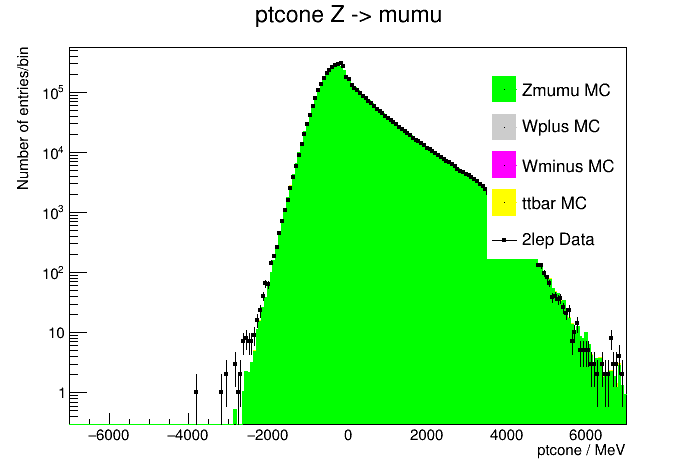
\includegraphics[width=0.85\linewidth]{plots/05-03-2021/11-30_05-03-21.png}
    \caption{\textbf{ETCone} with full cuts:}
    \label{fig:12-08_05-03-21}
\end{figure}


%%%%%%%%%%%%% 14:15 %%%%%%%%%%%%%
\subsubsection*{14:15 - Estimation of systematic uncertainty using variations in PT for $\sigma (Z \rightarrow \mu\mu)$}


%%%%%%%%%%%%% 15:35 %%%%%%%%%%%%%
\subsubsection*{15:35 - Estimation of systematic uncertainty using variations in invariant mass for $\sigma (Z \rightarrow \mu\mu)$}

Cuts used:
\begin{lstlisting}
basic_cut = "(lep_charge[0] != lep_charge[1]) && (lep_type[0] == 13 && lep_type[1] == 13) && lep_n==2"

etcone_cut = "(lep_etcone20[0] > -1.6e3 && lep_etcone20[1] > -1.6e3)" + "&& (lep_etcone20[0] < 5.25e3 && lep_etcone20[1] < 5.25e3)"

ptcone_cut = "(lep_ptcone30[0] < 6.5e3) && (lep_ptcone30[1] < 6.5e3)"

pt_cut = "(lep_pt[0] > 28e3) && (lep_pt[1] > 28e3)"
    
lepCut = "(" + basic_cut + "&&" + etcone_cut + "&&" + ptcone_cut + "&&" + pt_cut + ")"
    
t.SetAlias("inv_mass_Zll","sqrt(2*lep_pt[0]*lep_pt[1]*(cosh(lep_eta[0]-lep_eta[1])-cos(lep_phi[0]-lep_phi[1])))")
  
t.Draw("inv_mass_Zll >> h_inv_mass(200,40e3,200e3)", weighting + "*" + lepCut)
\end{lstlisting}


%%%%%%%%%%%%% 16:44 %%%%%%%%%%%%%
\subsubsection*{16:44 - Estimation of systematic uncertainty using variations in etcone20 for $\sigma (Z \rightarrow ee)$}
Cuts used in Fig.\ref{}:
\begin{lstlisting}
basic_cut = "(lep_charge[0] != lep_charge[1]) && (lep_type[0] == 11 && lep_type[1] == 11) && lep_n==2"
    inv_mass_cut = "(inv_mass_Zll > 65e3) && (inv_mass_Zll < 150e3)"

ptcone_cut = "(lep_ptcone30[0] < 5.8e3) && (lep_ptcone30[1] < 5.8e3)"
pt_cut = "(lep_pt[0] > 26e3) && (lep_pt[1] > 26e3)"
 
lepCut = "(" + basic_cut + "&&" + pt_cut + "&&" + inv_mass_cut + "&&" + ptcone_cut + ")"
    
t.SetAlias("inv_mass_Zll","sqrt(2*lep_pt[0]*lep_pt[1]*(cosh(lep_eta[0]-lep_eta[1])-cos(lep_phi[0]-lep_phi[1])))")
    
t.Draw("lep_etcone20[0] >> h_lep_etcone_e(200,-7e3,7e3)", weighting + "*" + lepCut)
\end{lstlisting}

\begin{figure}[h!]
    \centering
    \begin{minipage}{0.5\textwidth}
        \centering
        \includegraphics[width=\linewidth]{plots/05-03-2021/}
        (A)
    \end{minipage}\hfill
    \begin{minipage}{0.5\textwidth}
        \centering
        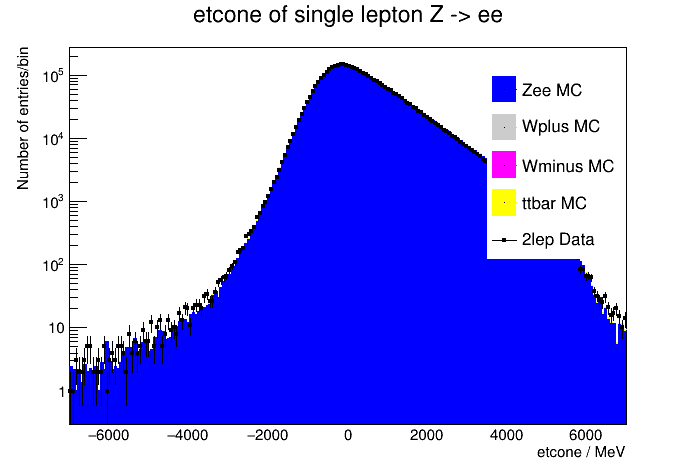
\includegraphics[width=\linewidth]{plots/05-03-2021/17-07_05-03-21.png}
        (B)
    \end{minipage}
    \caption{(A) etcone of single lepton for Z->ee (B) log-y.  Full Cuts.}
    \label{}
\end{figure}


%%%%%%%%%%%%% 17:07 %%%%%%%%%%%%%
\subsubsection*{17:07 - Estimation of systematic uncertainty using variations in ptcone30 for $\sigma (Z \rightarrow ee)$}
Cuts used in Fig.\ref{}:
\begin{lstlisting}
basic_cut = "(lep_charge[0] != lep_charge[1]) && (lep_type[0] == 11 && lep_type[1] == 11) && lep_n==2"
    inv_mass_cut = "(inv_mass_Zll > 65e3) && (inv_mass_Zll < 150e3)"
    etcone_cut = "(lep_etcone20[0] > -2e3 && lep_etcone20[1] > -2e3)" + "&& (lep_etcone20[0] < 6e3 && lep_etcone20[1] < 6e3)"
#     ptcone_cut = "(lep_ptcone30[0] < 6.5e3) && (lep_ptcone30[1] < 6.5e3)"
    pt_cut = "(lep_pt[0] > 26e3) && (lep_pt[1] > 26e3)"
    
    lepCut = "(" + basic_cut + "&&" + pt_cut + "&&" + inv_mass_cut + "&&" + etcone_cut + ")"

    t.SetAlias("inv_mass_Zll","sqrt(2*lep_pt[0]*lep_pt[1]*(cosh(lep_eta[0]-lep_eta[1])-cos(lep_phi[0]-lep_phi[1])))")
   
    t.Draw("lep_ptcone30[0] >> h_lep_ptcone30_e(100,0e3,7e3)", weighting + "*" + lepCut)
\end{lstlisting}

\begin{figure}[h!]
    \centering
    \begin{minipage}{0.5\textwidth}
        \centering
        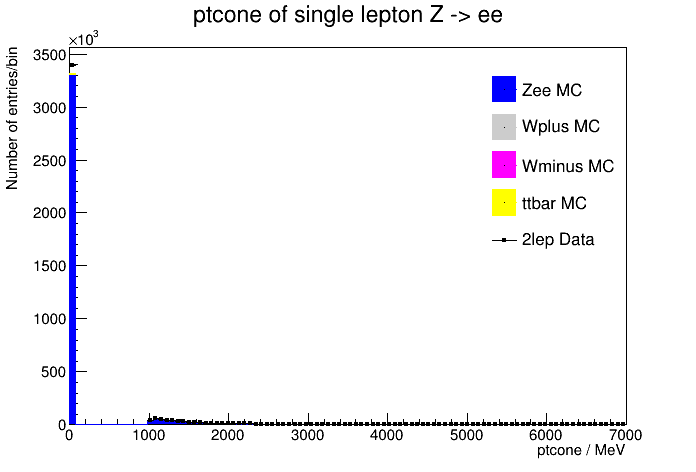
\includegraphics[width=\linewidth]{plots/05-03-2021/17-31_05-03-21.png}
        (A)
    \end{minipage}\hfill
    \begin{minipage}{0.5\textwidth}
        \centering
        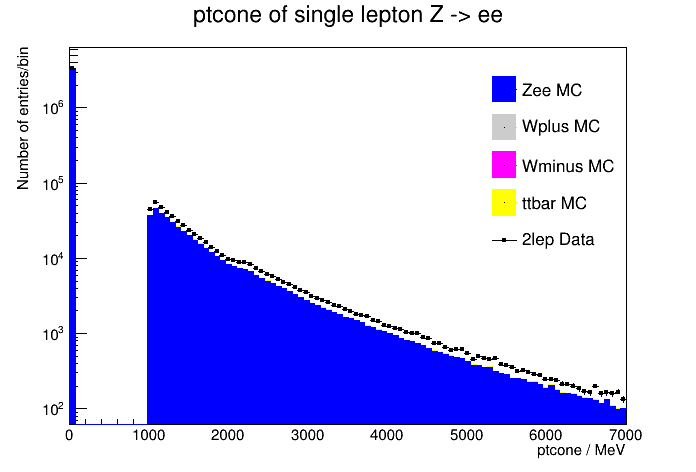
\includegraphics[width=\linewidth]{plots/05-03-2021/17-30_05-03-21.png}
        (B)
    \end{minipage}
    \caption{(A) ptcone single lep Z -> ee (B) ptcone single lep Z -> ee - log-y. full cuts }
    \label{}
\end{figure}

%%%%%%%%%%%%%%%%%%%%%%%%%%%%%%%%%%%%%%%%%%%%%%%%%%%%%%%%%%%%%%%%%%%%%%%%%%%%%%%%%%%%%%%%%%%%%%%%%%%%%%%%%%%%%%%%%%%%%%%%
% \begin{figure}[h!]
%     \centering
%     \begin{minipage}{0.5\textwidth}
%         \centering
%         \includegraphics[width=\linewidth]{plots/05-03-2021/}
%         (A)
%     \end{minipage}\hfill
%     \begin{minipage}{0.5\textwidth}
%         \centering
%         \includegraphics[width=\linewidth]{plots/05-03-2021/}
%         (B)
%     \end{minipage}
%     \caption{(A)  (B)}
%     \label{}
% \end{figure}
